\documentstyle[a4,11pt,epsfig]{jarticle}
\topmargin=-1.5cm
\textwidth=17cm
\textheight=25cm
\oddsidemargin=-0.5cm
\evensidemargin=-0.5cm

\begin{document}
\begin{center}
  \Large\bf 情報活用演習 課題9
\end{center}

\begin{flushright}
  \begin{tabular}{ll}
    学生番号: & B151235 \\
    氏名:     & 山下 直哉 \\
    提出日:   & 平成27年12月08日 \\
    提出期限: & 平成27年12月15日 \\
  \end{tabular}
\end{flushright}

\begin {center}
  まち・ひと・しごと創生 \\
  「長期ビジョン」「総合戦略」 \\
  内閣官房まち・ひと・しごと創生本部事務局 \\
\end {center}

\section {まち・ひと・しごと創生とは}
\subsection {まち・ひと・しごと創生が目指すもの}
\begin {itemize}
\item 2008 年に始まった人口減少は、今後加速度的に進む。\par
\item 人口減少による消費・経済力の低下は、日本の経済社会に対して大きな重荷となる。\par
\item 国民の希望を実現し、人口減少に歯止めをかけ、2060 年に1億人程度の人口を確保する。\par
\item まち・ひと・しごと創生は、人口減少克服と地方創生をあわせて行うことにより、 将来にわたって活力ある日本社会を維持することを目指す。\par

  \begin{figure}[htb]
    \begin{center}
      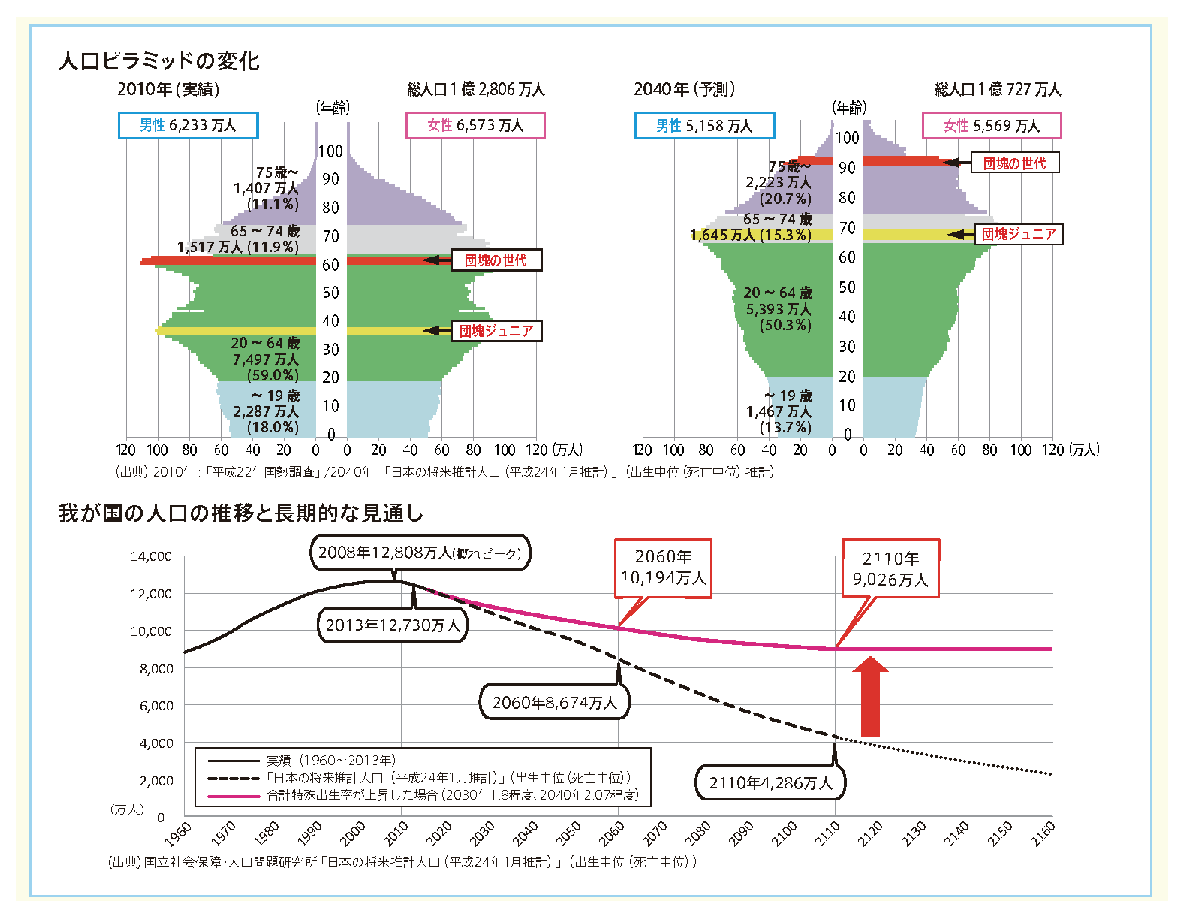
\epsfig{file=fig01.eps, width=14cm}
    \end{center}
  \end{figure}

\end {itemize}

\subsection {なぜ,まち・ひと・しごと創生か}
\begin {itemize}
\item 人口減少問題は地域によって状況や原因が異なる。
\item 大都市における超低出生率・地方における都市への 人口流出+低出生率が日本全体の人口減少
  につながっている。
\item 東京一極集中を是正し、若い世代の結婚・子育て 希望を実現することにより人口減少を克服。
\item 地域特性に応じた処方せんが必要。

  \begin{figure}[htb]
    \begin{center}
      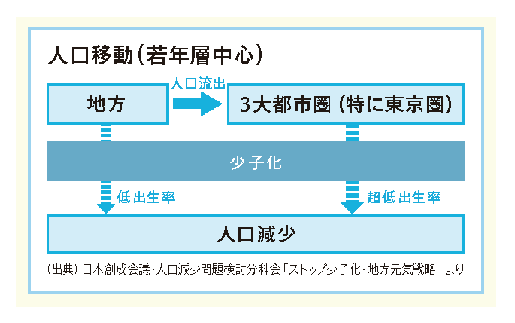
\epsfig{file=fig02.eps, width=6cm}
    \end{center}
  \end{figure}

\end {itemize}

\subsection {地方への多様な支援と「切れ目」のない施策の展開}
\begin{figure}[htb]
  \begin{center}
    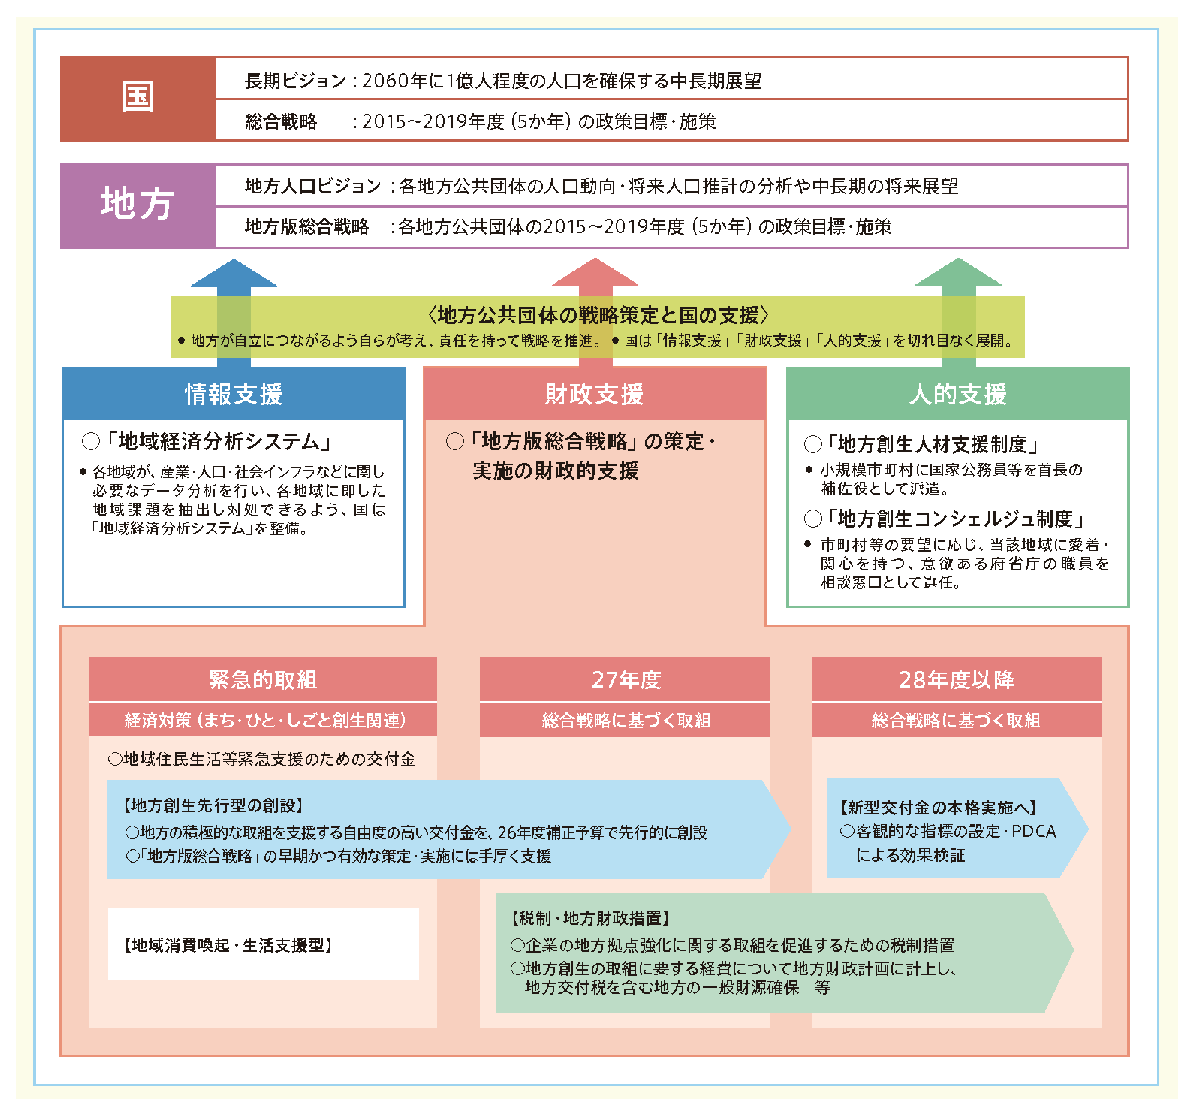
\epsfig{file=fig03.eps, width=16cm}
  \end{center}
\end{figure}

\subsection {「地方人口ビジョン」・「地方版総合戦略」策定のポイント}
\begin {itemize}
\item すべての都道府県及び市町村は、平成27 年度中に「地方人口ビジョン」「地方版総合戦略」の策定に努める。
\item 地域経済分析システム(ビッグデータ)等を活用し、地域特性を把握した効果的な政策立案。
\item 明確な目標とKPI ※ 1(重要業績評価指標)を設定し、PDCAサイクル※ 2 による効果検証・改善。
\item 地方公共団体を含め、産官学金労言※ 3、女性、若者、高齢者などあらゆる人の協力・参画を促す。
\item 地方議会も策定や検証に積極的に関与。
\item 各々の地域での自律的な取組と地域間連携の推進。
\end {itemize}

\section {長期ビジョン・総合戦略}
\subsection {長期ビジョン}
\begin {itemize}
\item 人口問題に対する基本認識
  「人口減少時代の到来」
\item 今後の基本的視点
  \begin {itemize}
  \item 3 つの基本的視点
    \begin {itemize}
    \item 「東京一極集中」の是正
    \item 若い世代の就労・結婚・子育ての希望の実現
    \item 地域の特性に即した地域課題の解決
    \end {itemize}
  \item 国民の希望の実現に全力を注ぐことが重要
  \end {itemize}
\item 目指すべき将来の方向
  将来にわたって「活力ある日本社会」を維持する
  \begin {itemize}
  \item 若い世代の希望が実現すると、出生率は1.8 程度に向上する。
  \item 人口減少に歯止めがかかると、2060 年に1 億人程度の人口が確保される。
  \item 人口構造が「若返る時期」を迎える
  \item 「人口の安定化」とともに「生産性の向上」が図られると、2050 年代に実質GDP 成長率は、1.5-2%程度に維持される。
  \end {itemize}
\item 地方創生がもたらす日本社会の姿
  \begin {itemize}
  \item 地方創生が目指す方向
    \begin {itemize}
    \item 自らの地方資源を活用した、多様な地域社会の形成を目指す。
    \item 外部との積極的なつながりにより、新たな視点から活性化を図る。
    \item 地方創生が実現すれば、地方が先行して若返る。
    \item 東京圏は、世界に開かれた「国際都市」への発展を目指す。
    \end {itemize}
    地方創生は、日本の創生であり、地方と東京圏がそれぞれの強みを活かし、日本全体を引っ張っていく
  \end {itemize}
\end {itemize}

\subsection {総合戦略}
\begin{figure}[htb]
  \begin{center}
    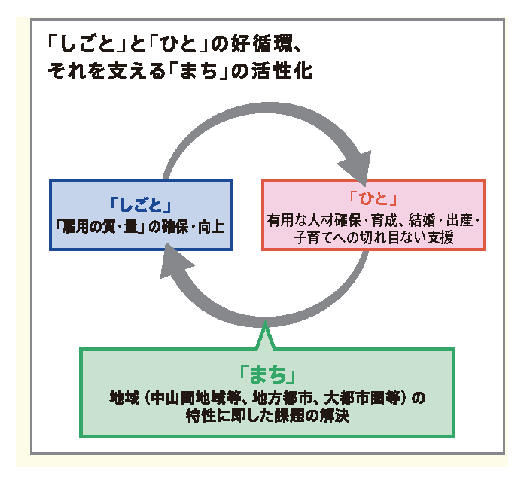
\epsfig{file=fig04.eps, width=8cm}
  \end{center}
\end{figure}

\begin {itemize}
\item 基本的な考え方
  \begin {itemize}
  \item 人口減少と地域経済縮小の克服
  \item まち・ひと・しごとの創生と好循環の確立
    「しごと」が「ひと」を呼び、「ひと」が「しごと」を呼び込む好循環を確立するとともに、その好循環を支える「まち」に活力を取り戻す。
  \end {itemize}
\item 政策の企画・実行に当たっての基本方針
  begin {itemize}
\item 政策5 原則
  従来の施策(縦割り、全国一律、バラマキ、表面的、短期的) の検証を踏まえ、政策5 原則(自立性、将来性、地域性、直接性、結果重視) に基づき施策展開。
\item 国と地方の取組体制とPDCA の整備
  国と地方公共団体とともに、5 か年の戦略を策定・実行する体制を整え、アウトカム指標を原則としたKPI で検証・改善する仕組みを確立。
\end {itemize}

\begin {itemize}
\item 今後の施策の方向
  \begin {itemize}
  \item 基本目標1: 地方における安定した雇用を創出する
  \item 基本目標2: 地方への新しいひとの流れをつくる
  \item 基本目標3: 若い世代の結婚・出産・子育ての希望をかなえる
  \item 基本目標4: 時代に合った地域をつくり、安心な暮らしを守るとともに、地域と地域を連携する
  \end {itemize}
\item 国家戦略特区・社会保障制度・税制・地方財政等
\end {itemize}

\section {基本目標1: 地方における安定した雇用を創出する}
\subsection {現状・課題}
\begin {itemize}
\item 2013 年の転入超過数の状況を見ると、東京圏では10 万人の転入超過となっており、その大半は10
  代後半~20 代の若者
\item 東京圏への人口移動は、経済・雇用情勢の格差が影響しており、地方における雇用創出が東京一極
  集中是正につながる
\end {itemize}

\subsection{基本目標}
地方において若者向けの雇用をつくる。2020 年までの5 年間で30 万人分
\begin {itemize}
\item 若い世代における正規雇用労働者の割合の向上。
\item 女性の就業率の向上。
\end {itemize}

\section {基本目標2: 地方への新しいひとの流れをつくる}
\subsection {現状・課題}
\begin {itemize}
\item 人口流入によって東京圏に人口が集中
\item 国際的に見ても首都圏への人口集中の割合が高く、さらに上昇傾向にある
\item 地方は人口減少の著しい地域が発生する見込み
\end {itemize}

\begin{figure}[htb]
  \begin{center}
    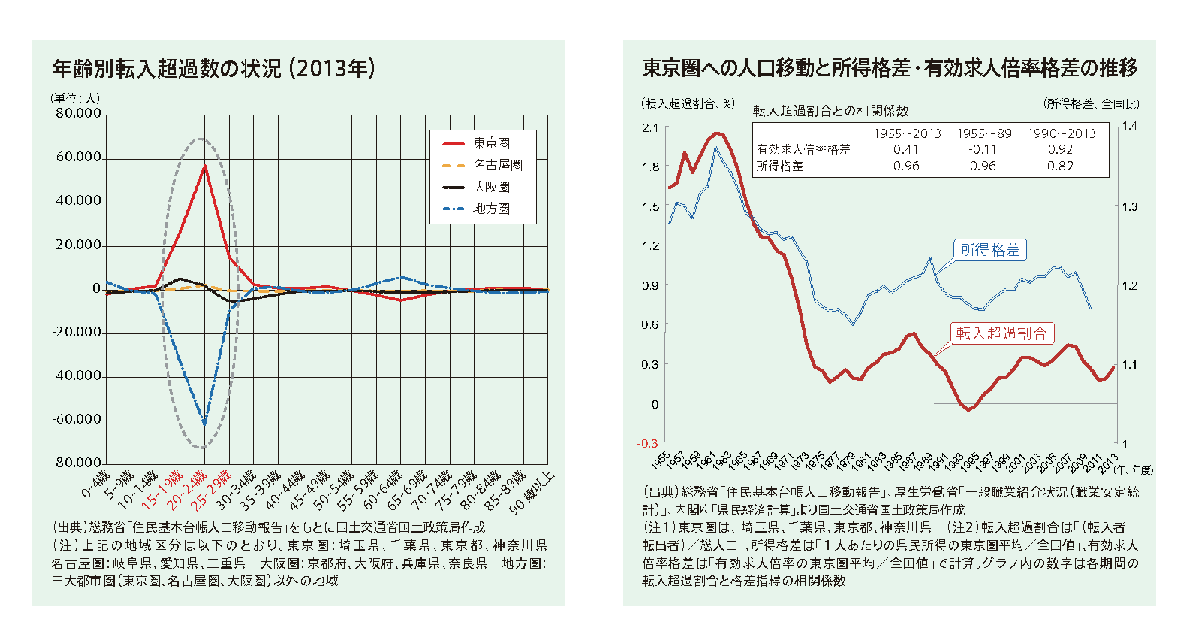
\epsfig{file=fig05.eps, width=8cm}
  \end{center}
\end{figure}

\subsection {基本目標}
現状で年間10 万人超の東京圏への人口流入に歯止めをかけ、東京圏と地方の人口の転出入を均衡させる
\begin {itemize}
\item 2020 年までに、東京圏から地方への転出を4 万人増加。
\item 2020 年までに、地方から東京圏への転入を6 万人減少。
\end {itemize}

\section {基本目標3: 若い世代の結婚・出産・子育ての希望をかなえる}
\subsection {現状・課題}
\begin {itemize}
\item 出生数は大きく減少 
\item 就労形態(非正規雇用等)は配偶者の有無の割合に大きく影響
\item ○未婚者の結婚意思は、9 割程度の高い水準・理想の子どもの数も2 名以上。一方、合計特殊出生率は1.43 となっており、理想と現実のギャップが存在
\end {itemize}

\begin{figure}[htb]
  \begin{center}
    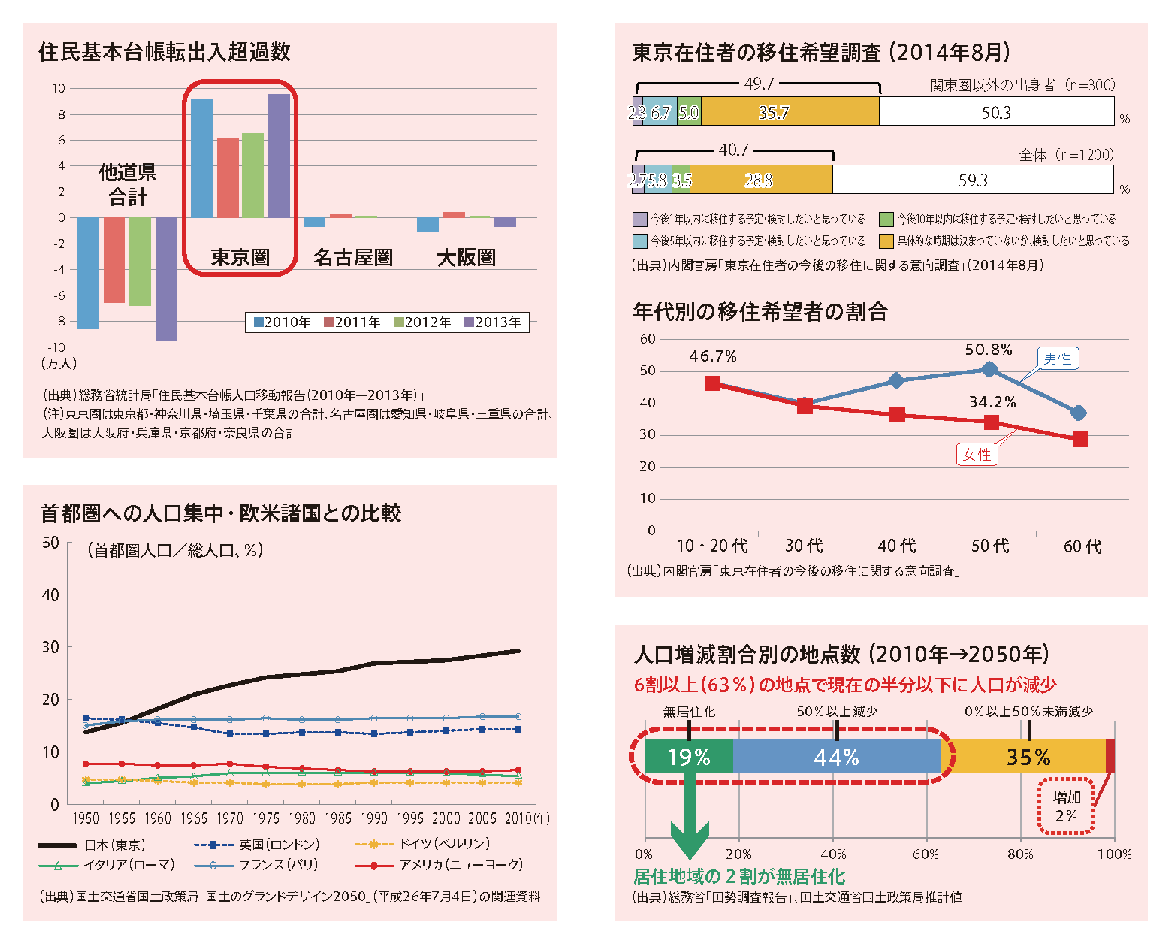
\epsfig{file=fig06.eps, width=8cm}
  \end{center}
\end{figure}


\subsection {基本目標}
若い世代が、安心して結婚・妊娠・子育てできるようにする
\begin {itemize}
\item 第1子出産前後の女性の継続就業率の向上。
\item 結婚希望実績指標の向上。
\item 夫婦子ども数予定実績指標の向上。
\end {itemize}

\section {基本目標4: 時代に合った地域をつくり,安全なくらしを守るとともに,地域と地域を連携する}
\subsection {現状・課題}
\begin {itemize}
\item 中山間地域・地方都市における人口減少に伴う生活サービス提供等、地域の維持・活性化への対応
\item 大都市における高齢化・単身化による医療・介護ニーズの拡大への対応
\item 老朽インフラ、空き家対応などストック対策
\item コミュニティ、ふるさとづくりへの対応
\end {itemize}

\subsection {基本目標}
            「小さな拠点」の整備や「地域連携」の推進

            \end{document}

